\section{Evaluierung und Ergebnisse}\label{sec:evaluation}

In diesem Abschnitt werden die Ergebnisse der Evaluierung des entwickelten \ac{poc} vorgestellt. Zunächst wird die technische Machbarkeit anhand des physischen Prototyps überprüft (Abschnitt~\ref{sec:poc}), anschließend werden die im Betrieb aufgetretenen Probleme und Lösungsansätze dokumentiert (Abschnitt~\ref{sec:problems}). Darauf aufbauend wird die Durchführung der szenariobasierten Kosten-Nutzen-Analyse mit ihren Annahmen erläutert und schließlich werden die berechneten Kennzahlen dargestellt und im Kontext der Forschungsfrage interpretiert (Abschnitt~\ref{sec:results}). Ziel ist es, sowohl die technische Umsetzbarkeit als auch die Wirtschaftlichkeit des vorgeschlagenen \ac{sps} zu bewerten und daraus Schlussfolgerungen für die Praxis abzuleiten.

\subsection{Evaluierung des Proof of Concept}\label{sec:poc}

Die Evaluierung des \ac{poc} diente dazu, die technische Grundannahme der Arbeit zu überprüfen: Ein einzelner Stellplatzwechsel sollte durch einen Sensor erkannt, vom Mikrocontroller verarbeitet und als Ereignis an die Cloud-Infrastruktur übertragen werden können. Damit sollte gezeigt werden, dass der in Abschnitt~\ref{sec:technical-setup} beschriebene Versuchsaufbau nicht nur konzeptionell, sondern auch praktisch umsetzbar ist.

Für den physischen Prototyp wurden mehrere Stellplätze eines Parkgaragenmodells mit \ac{ir}-Sensoren des Modells TCRT5000 ausgestattet. Die \ac{ir}-Sensoren wurden an einen ESP32-Mikrocontroller angeschlossen, der über \ac{wlan} verbunden war. Bei einer Änderung des Belegungsstatus wurde eine \ac{mqtt}-Nachricht erzeugt und an ein strukturiertes Topic nach dem Schema \texttt{parking/garage1/spot/\{spotId\}} veröffentlicht. Die Nachrichten enthielten die Sensor-ID, eine Garagen-ID, eine Stellplatz-ID, einen Zeitstempel, den Rohwert des Sensors und den daraus abgeleiteten Status.

Die Tests zeigten, dass Belegungsänderungen einzelner Stellplätze grundsätzlich erkannt wurden. Wird ein Fahrzeug auf einen Stellplatz gestellt oder entfernt, erkennt der jeweilige Sensor die Änderung des Rohwertes und der ESP32 leitet daraus den Status \texttt{occupied} oder \texttt{free} ab. Die Ausgabe über die serielle Schnittstelle bestätigte, dass Statusänderungen nur bei tatsächlichen Zustandswechseln veröffentlicht wurden. Dadurch wurde ein ereignisgetriebener Datenfluss umgesetzt, der unnötige Nachrichten vermeidet und damit die Grundlage für eine nutzungsabhängige Kostenmodellierung bildet.

Auch die Übertragung an \ac{aws} IoT Core wurde erfolgreich getestet. Die \ac{mqtt}-Nachricht wurde auf dem definierten Topic veröffentlicht und in der Cloud weiterverarbeitet. Der \ac{aws} IoT Core Test Client sowie die in der DynamoDB-Tabelle gespeicherten Items dienten dabei als Indikatoren für die erfolgreiche Übertragung und Verarbeitung. Damit wurde gezeigt, dass der gewählte Aufbau aus Sensorik, ESP32, \ac{wlan}, \ac{mqtt} und \ac{aws} IoT Core die grundlegende technische Voraussetzung für ein \ac{sps} erfüllt.

Zusammenfassend bestätigt der \ac{poc} die technische Machbarkeit des entwickelten Ansatzes. Der Prototyp konnte Stellplatzänderungen erkennen, in strukturierte Ereignisdaten umwandeln und über \ac{mqtt} an die \ac{aws}-basierte Cloud-Infrastruktur übertragen. Damit bildet er eine geeignete Grundlage für die anschließende Bewertung der Skalierbarkeit und Wirtschaftlichkeit.

\subsection{Aufgetretene Probleme und Lösungsansätze}\label{sec:problems}

Im praktischen Betrieb des physischen Prototyps traten mehrere Herausforderungen auf, die für die Bewertung der technischen Reife relevant sind.

\textbf{Verbindungsabbrüche.} Die Anbindung des ESP32 über \ac{wlan} war zeitweise instabil. Abbrüche der \ac{wlan}- oder \ac{mqtt}-Verbindung führten dazu, dass einzelne Statusänderungen nicht übertragen wurden, wobei die Ursache des Verbindungsabbruchs nicht geklärt werden konnte. Als Lösung wurde in der Firmware eine automatische Wiederverbindung implementiert, die sowohl die \ac{wlan}- als auch die \ac{mqtt}-Verbindung bei einem Abbruch erneut aufbaut, bevor weitere Nachrichten gesendet werden. Verbindungsabbrüche und der erneute Verbindungsaufbau wurden außerdem für die zukünftige Problembehebung in der Konsole geloggt.

\textbf{Schwankende Sensorwerte (\enquote{Flackern}).} Die reflexionsbasierte Messung des TCRT5000 hängt von der Beschaffenheit der Fahrzeugunterseite ab. Das \enquote{Flackern} beschreibt mehrfach ausgelöste Statusänderungen durch ein bewegtes Fahrzeug, bei dem das Licht vom Unterboden des Fahrzeugs unterschiedlich gut zurückgeworfen wird. Auslöser dafür könnten die Unebenheit sowie eine zu helle oder zu dunkle Lackierung gewesen sein. Testweise wurden daher weiße Sticker aufgeklebt, um eine gleichmäßige Fläche und Farbe zu bieten, wodurch kurzfristig Verbesserungen bei der Messgenauigkeit erzielt werden konnten. Die Verlässlichkeit dieses Workarounds sowie die Ursache sollten jedoch weiter untersucht werden. Zusätzlich könnte in der Firmware ein Schwellenwert implementiert werden, bei dem der Status erst dann abgesendet wird, wenn dieser Wert nach einer Änderung über mehrere Sekunden unverändert bleibt.

\textbf{Messempfindlichkeit.} Der TCRT5000 erfasst Objekte nur in einem lokal begrenzten, winkelabhängigen Bereich. Die Sensoren wurden aus Designgründen in den Boden des Modells eingelassen. Fahrzeuge, die nicht mittig über diesem Bereich standen, wurden nicht zuverlässig erkannt. Je tiefer der Sensor gelegt wurde, desto eher wurde außerdem das Licht seitlich vom Boden zurückgeworfen und eine fälschliche Statusänderung ausgesendet. Somit musste der Sensor leicht über die Oberfläche des Bodens hinausragen.

\textbf{Lichtverhältnisse.} Wechselnde Umgebungslichtverhältnisse, insbesondere Sonnenlicht, können reflexionsbasierte \ac{ir}-Sensoren beeinflussen. Im Modellbetrieb war dieser Effekt erkennbar, weshalb Versuche besonders in lichtarmer Umgebung durchgeführt wurden. Für einen realen Außeneinsatz wären eine robustere Sensorik (etwa \ac{tof}-Sensoren) zu prüfen, oder mehrere Sensoren für genauere Messungen zu kombinieren.

Diese Beobachtungen bestätigen die in der Literatur beschriebenen Eigenschaften kostengünstiger reflexionsbasierter Sensoren \citep{perkovicSmartParkingSensors2020} und fließen als qualitative Einordnung in die Bewertung ein.

\subsection{Durchführung der Evaluierung}

Die wirtschaftliche Evaluierung wurde als szenariobasierte Kosten-Nutzen-Analyse durchgeführt. Da keine vollständigen, öffentlich zugänglichen Echtzeitdaten zu Auslastung, Umsatz und Umschlaghäufigkeit einzelner Wiener Parkhäuser vorlagen, wurden die gewählten Einflussgrößen als transparente Modellparameter definiert. Die verwendeten Werte dienen daher nicht als exakte Abbildung eines konkreten Parkhauses, sondern als nachvollziehbare Annahmen für einen typischen urbanen Parkhausbetrieb. Sämtliche Annahmen sind in Tabelle~\ref{tab:assumptions} mit Quellen zusammengefasst.

\subsubsection{Datenbasis und Szenariodefinition}

Als Grundlage für die Szenariodefinition wurde Wien als Referenzstadt gewählt. Die Größe der betrachteten Parkgarage wurde aus öffentlich verfügbaren Informationen zum Wiener Parkleitsystem abgeleitet \citep{stadtwienParkleitsystemFuerWien2026}. Bei aktuell 128 eingebundenen Parkhäusern und Garagen und insgesamt 53.200 Stellplätzen ergibt sich eine durchschnittliche Größe von rund 416 Stellplätzen pro Parkhaus. Ein kleineres Szenario mit 200 Stellplätzen, ein Basisszenario mit 400 Stellplätzen und ein größeres Szenario mit 500 Stellplätzen entsprechen damit der in Abschnitt~\ref{sec:methodology} beschriebenen Definition eines mittelgroßen Wiener Parkhausbetreibers.

\subsubsection{Technische und wirtschaftliche Messgrößen des Prototyps}

Für die technische Evaluierung wurden die Statusänderungen der Stellplätze im physischen Prototyp beobachtet. Bewertet wurde, ob ein Wechsel zwischen \texttt{free} und \texttt{occupied} durch den Sensor erkannt, vom ESP32 verarbeitet und als \ac{mqtt}-Nachricht an \ac{aws} IoT Core übertragen wurde. Zusätzlich wurde überprüft, ob die übermittelten Nachrichten die vorgesehenen Attribute (Sensor-ID, Stellplatz-ID, Zeitstempel, Rohwert und Status) enthielten.

Für die wirtschaftliche Evaluierung wurde der physische Prototyp als Funktionsnachweis verwendet und das resultierende Lastverhalten anschließend auf größere Szenarien skaliert. Da der ereignisgetriebene Aufbau ausschließlich Zustandswechsel überträgt, entspricht ein Parkvorgang mindestens zwei Cloud-Ereignissen: einer Statusänderung von \texttt{free} auf \texttt{occupied} beim Einparken und einer von \texttt{occupied} auf \texttt{free} beim Ausparken. Um realistische Lastmengen ohne den Aufbau hunderter Sensoren zu erhalten, wurde die Last mit dem virtuellen Prototyp (Lastgenerator) erzeugt: Dieser simuliert für eine definierte Stellplatzzahl ein Belegungsprofil und protokolliert die erzeugten Nachrichten in einem Lauf-Manifest. Aus diesem Manifest wurde die mittlere Ereignisrate je Stellplatz und Tag abgeleitet (rund 27 Ereignisse je Stellplatz und Tag im betrachteten Lastprofil), die als Eingangsgröße für die Hochrechnung der \ac{aws}-Nutzung dient.

\subsubsection{Kostenannahmen}

Die Kostenseite wurde in \ac{capex} und \ac{opex} unterteilt. Für die \ac{capex} wurden die Kosten für Sensoren, Mikrocontroller, Verkabelung, Installation und initiale Cloud-Konfiguration herangezogen. Für die \ac{opex} wurden zwei Treiber getrennt modelliert: erstens die schreibseitigen, nutzungsabhängigen \ac{aws}-Kosten je Belegungsereignis (IoT Core, Validierungs-Lambda und DynamoDB-Schreibvorgang) und zweitens die leseseitigen Kosten der Datenabfrage (\ac{api} Gateway, Aggregations-Lambda und DynamoDB-Lesevorgänge), die durch die Abfragefrequenz der Konsumenten bestimmt werden. Ergänzt wurden Datentransfer, Speicher sowie nicht-cloudbezogene Kosten für Wartung, Sensoraustausch und Stromverbrauch. Die \ac{aws}-Stückpreise wurden den offiziellen Preislisten entnommen\footnote{\url{https://aws.amazon.com/iot-core/pricing/}, \url{https://aws.amazon.com/lambda/pricing/}, \url{https://aws.amazon.com/dynamodb/pricing/on-demand/} (Stand 2026-06, Region eu-central-1, Umrechnung USD/EUR zu 1{,}08).}, die Hardwarekosten aus Herstellerangaben und Online-Shops sowie der Installationsaufwand aus einem aktuellen Stundensatzvergleich für Elektroinstallation\footnote{Arbeiterkammer Oberösterreich, Preisvergleich Elektromonteure (Mai 2025): \url{https://ooe.arbeiterkammer.at/service/testsundpreisvergleiche/preisvergleiche/Preisvergleich-Elektromonteure.html}.} abgeleitet. Der Stromverbrauch wurde aus dem kommerziellen österreichischen Strompreis berechnet\footnote{E-Control / GlobalPetrolPrices (September 2025): 0{,}247\,EUR/kWh, \url{https://www.globalpetrolprices.com/Austria/electricity_prices/}.}.

% Die Kostenseite wurde in \ac{capex} und \ac{opex} unterteilt. Für die \ac{capex} wurden die Kosten für Sensoren, Mikrocontroller, Verkabelung, Installation und initiale Cloud-Konfiguration herangezogen. Für die \ac{opex} wurden die nutzungsabhängigen \ac{aws}-Kosten für IoT Core, Lambda, DynamoDB, Datentransfer und Speicher sowie Wartung, Sensoraustausch und Stromverbrauch berücksichtigt. \ac{aws}-Kosten wurden mithilfe des \ac{aws} Pricing Calculators und offiziellen Preislisten ermittelt. Hardwarespezifische Kosten wurden von Herstellerangaben und Online-Shops abgeleitet. 
% % Wartungskosten wurden auf Basis von Erfahrungswerten aus der IT- und Sensorikbranche geschätzt.

\subsubsection{Nutzenannahmen}

Die Nutzenseite wurde primär über eine bessere Auslastung modelliert: Eine zuverlässigere Auffindbarkeit freier Stellplätze führt zu zusätzlichen belegten Stellplatzstunden, die mit dem Parktarif bewertet werden. Der modellierte Mehrerlös ergibt sich somit aus der Auslastungssteigerung (in Prozentpunkten), der Stellplatzzahl, dem Tarif je Stellplatzstunde und den jährlichen Betriebsstunden. Da die tatsächliche Auslastungssteigerung eines konkreten Parkhauses nicht bekannt ist, wurde sie als Sensitivitätsparameter behandelt und in einem konservativen (+1\,pp), einem mittleren (+3\,pp) und einem optimistischen (+6\,pp) Szenario betrachtet \citep{wangEconomicsSmartParking2025,sarkerSmartParkingSystem2020}. Der Parktarif wurde anhand realer Wiener Garagentarife plausibilisiert\footnote{WIPARK Wien (2026), z.\,B. Beethovenplatz 4{,}90\,EUR/h, TU Operngasse 4{,}70\,EUR/h: \url{https://www.wipark.at/standorte}.}. Als ergänzender, additiver Nutzenpfad wurde ein moderater Mehrerlös durch dynamische Preisgestaltung in Stoßzeiten berücksichtigt \citep{hassineDynamicPricingRoute2024}. Die weiteren in Abschnitt~\ref{sec:methodology} genannten Nutzenpotenziale (reduzierte Fehlfahrten und Reputationseffekte sowie die Verwertung anonymisierter Auslastungsdaten) wurden bewusst nicht monetarisiert, um eine Überschätzung des Nutzens zu vermeiden; sie werden qualitativ eingeordnet.

Die Wirtschaftlichkeit wurde anhand von \ac{tco}, \ac{roi}, Amortisationsdauer und Break-Even-Punkt beurteilt. Der Break-Even-Punkt ist dabei besonders relevant, da er die notwendige Auslastungssteigerung in Prozentpunkten angibt, ab der sich die Investition trägt, und damit unabhängig von einer einzelnen unterstellten Nutzenannahme bewertet werden kann.

\subsubsection{Berechnung der Kennzahlen}

Die Kennzahlen wurden mit einem reproduzierbaren Modell berechnet, das sämtliche Eingangsgrößen aus einer dokumentierten Parameterdatei bezieht. Die \ac{capex} ergeben sich aus den Stückkosten je Stellplatz (Sensor, Verkabelung, Installation), den stufenweise mit der Stellplatzzahl wachsenden Kosten der Mikrocontroller-Knoten sowie den einmaligen Fixkosten für Netzwerk und Cloud-Einrichtung. Die jährlichen \ac{opex} setzen sich aus den beschriebenen schreib- und leseseitigen \ac{aws}-Kosten und den nicht-cloudbezogenen Kosten zusammen. Die \ac{tco} über den Betrachtungszeitraum von fünf Jahren ergeben sich aus den \ac{capex} zuzüglich der kumulierten \ac{opex}.

Der jährliche Mehrerlös wird, wie in den Nutzenannahmen beschrieben, aus der Auslastungssteigerung und dem Tarif berechnet. Der \ac{roi} setzt den kumulierten Mehrerlös über fünf Jahre ins Verhältnis zu den \ac{tco}, die Amortisationsdauer ergibt sich aus dem Verhältnis von Investition zu jährlichem Netto-Mehrerlös. Der Break-Even-Punkt invertiert den Auslastungs-Nutzenpfad und gibt jene Auslastungssteigerung in Prozentpunkten an, bei der der Mehrerlös die Kosten gerade deckt. Eine einfache Sensitivitätsanalyse variiert abschließend die wichtigsten Parameter um $\pm$30\,\%, um deren Einfluss auf das Ergebnis zu bestimmen.

\subsection{Ergebnisse und Interpretation der Evaluierung}\label{sec:results}

Tabelle~\ref{tab:assumptions} fasst die zentralen Modellannahmen mit ihren Quellen zusammen. Tabelle~\ref{tab:results} zeigt die berechneten Kennzahlen für die drei Garagengrößen im Basisszenario (+3\,pp Auslastungssteigerung).

\begin{table}[!ht]
  \centering
  \caption{Zentrale Modellannahmen der Kosten-Nutzen-Analyse}
  \label{tab:assumptions}
  \begin{tabular}{lll}
    \toprule
    Parameter & Wert & Quelle \\
    \midrule
    Betrachtungszeitraum & 5 Jahre & Methodik \\
    Stellplatzszenarien & 200 / 400 / 500 & \citep{stadtwienParkleitsystemFuerWien2026} \\
    Sensor (TCRT5000) & 0{,}80\,EUR & Vendor \\
    Mikrocontroller (ESP32) & 12\,EUR & Vendor \\
    Installation & 16\,EUR/Stellplatz & AK OÖ 2025 \\
    Parktarif & 4{,}50\,EUR/h & WIPARK 2026 \\
    Basisauslastung & 75\,\% & \citep{wangEconomicsSmartParking2025} \\
    Auslastungssteigerung & +1 / +3 / +6\,pp & \citep{wangEconomicsSmartParking2025,sarkerSmartParkingSystem2020} \\
    Dyn.\ Preisaufschlag & +2\,\% & \citep{hassineDynamicPricingRoute2024} \\
    AWS-Stückpreise & Listenpreise eu-central-1 & AWS 2026 \\
    Strompreis & 0{,}247\,EUR/kWh & E-Control 2025 \\
    Ereignisrate & $\approx$27 je Stellplatz/Tag & Lastgenerator \\
    \bottomrule
  \end{tabular}
\end{table}

\begin{table}[!ht]
  \centering
  \caption{Berechnete Kennzahlen je Szenario (Basisfall, +3\,pp)}
  \label{tab:results}
  \begin{tabular}{lrrrr}
    \toprule
    Szenario & Stellpl. & CAPEX & OPEX/Jahr & Break-Even \\
             &          & (EUR)  & (EUR)     & ($\Delta$pp) \\
    \midrule
    Klein & 200 & 7.616  & 468 & 0{,}04 \\
    Basis & 400 & 11.720 & 748 & 0{,}03 \\
    Groß  & 500 & 13.784 & 891 & 0{,}03 \\
    \bottomrule
  \end{tabular}
\end{table}

Über alle drei Garagengrößen liegen die einmaligen Investitionskosten zwischen rund 7.600\,EUR (200 Stellplätze) und 13.800\,EUR (500 Stellplätze); die laufenden Betriebskosten betragen lediglich rund 470 bis 890\,EUR pro Jahr. Der geringe \ac{opex}-Anteil bestätigt eine zentrale Annahme der Arbeit: Der durchgehend ereignisgetriebene, serverlose Aufbau verursacht im Verhältnis zu den potenziellen Parkerlösen nur sehr geringe laufende Cloud-Kosten. Die Kostenstruktur (Abbildung~\ref{fig:cost_breakdown}) wird damit klar von den einmaligen \ac{capex} dominiert.

Das wichtigste Ergebnis ist der Break-Even-Punkt: Schon eine Auslastungssteigerung von rund 0{,}03 bis 0{,}04 Prozentpunkten reicht aus, damit sich das System rechnet (Abbildung~\ref{fig:breakeven}). Dieser Wert liegt deutlich unter dem konservativsten betrachteten Szenario (+1\,pp) und unter den in der Literatur berichteten Effekten von Smart-Parking-Systemen \citep{wangEconomicsSmartParking2025}. Damit amortisiert sich die Investition unter den hier angenommenen Bedingungen; entsprechend sind \ac{roi} und Amortisationsdauer über alle Szenarien hinweg deutlich positiv bzw.\ liegen weit innerhalb des ersten Betriebsjahres.

Die Sensitivitätsanalyse (Abbildung~\ref{fig:tornado}) zeigt, dass das Ergebnis nahezu vollständig von der Nutzenseite bestimmt wird: Der Parktarif und die unterstellte Auslastungssteigerung haben den mit Abstand größten Einfluss, während die Sensor-Stückkosten und die Cloud-Ereignisrate kaum eine Rolle spielen. Dies unterstreicht, dass die Aussagekraft der Wirtschaftlichkeitsbetrachtung an den Nutzenannahmen hängt -- und begründet, warum der Break-Even-Punkt und nicht ein einzelner \ac{roi}-Wert als belastbare Kennzahl berichtet wird.

\begin{figure}[!ht]
  \centering
  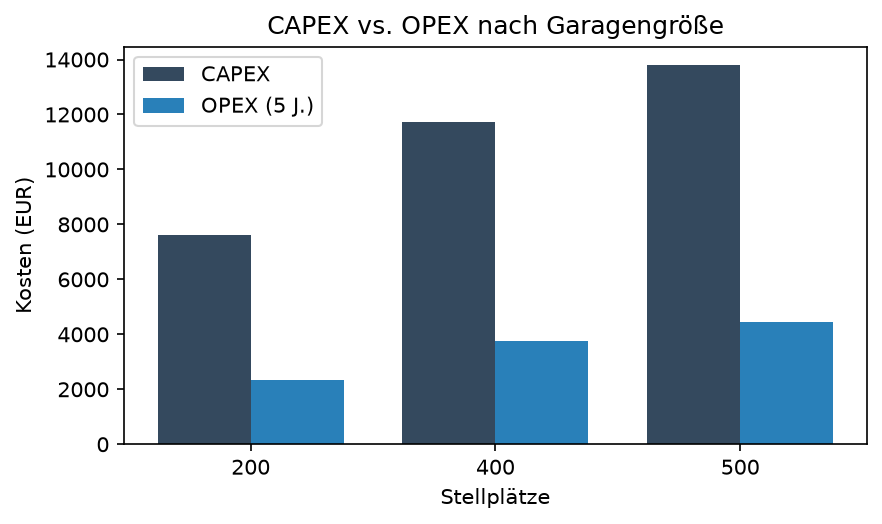
\includegraphics[width=\linewidth]{fig/cost_breakdown.png}
  \caption{Kostenstruktur (CAPEX vs.\ kumulierte OPEX über 5 Jahre) je Szenario}
  \Description[Kostenstruktur]{Balkendiagramm der CAPEX und OPEX je Szenario}
  \label{fig:cost_breakdown}
\end{figure}

\begin{figure}[!ht]
  \centering
  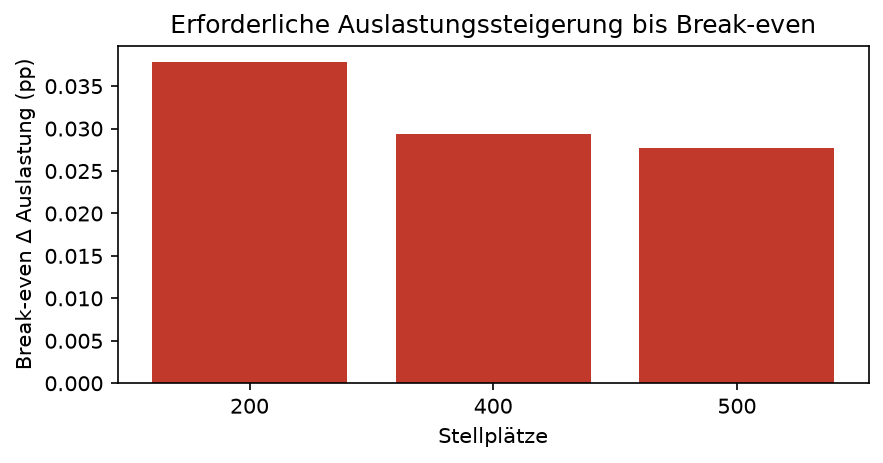
\includegraphics[width=\linewidth]{fig/breakeven_uplift.png}
  \caption{Break-Even-Auslastungssteigerung im Vergleich zu den Szenarien}
  \Description[Break-Even]{Break-Even-Auslastungssteigerung je Szenario}
  \label{fig:breakeven}
\end{figure}

\begin{figure}[!ht]
  \centering
  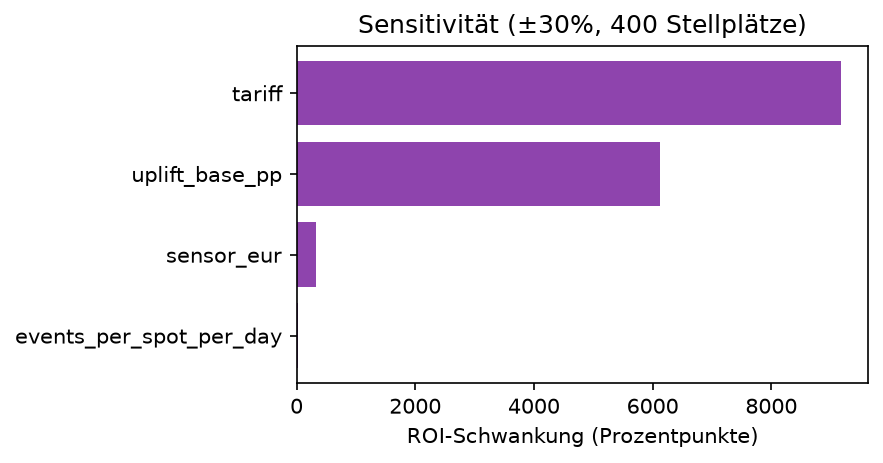
\includegraphics[width=\linewidth]{fig/sensitivity_tornado.png}
  \caption{Einfluss der wichtigsten Parameter auf den ROI ($\pm$30\,\%)}
  \Description[Sensitivität]{Tornado-Diagramm der Parametereinflüsse auf den ROI}
  \label{fig:tornado}
\end{figure}
\FloatBarrier

\textbf{Einschränkungen.} Die Ergebnisse beruhen auf modellierten und nicht auf über einen längeren Zeitraum gemessenen Cloud-Kosten; eine kurze gemessene Vergleichsmessung in \ac{aws} steht noch aus. Zudem unterstellt das Nutzenmodell, dass jede zusätzliche Auslastung über die gesamte Betriebszeit zum vollen Stundentarif erlösbar ist, was den Nutzen tendenziell überschätzt. Aus diesem Grund sind die rechnerisch sehr hohen \ac{roi}-Werte und die nahezu sofortige Amortisation nicht als exakte Prognose, sondern als Bestätigung der Größenordnung zu verstehen; die belastbare Aussage liefert der Break-Even-Punkt. Schließlich bilden die offen dokumentierten Annahmen einen typischen Betrieb ab und sind für andere Betreiberprofile entsprechend anzupassen.

Insgesamt belegt die Evaluierung sowohl die technische Machbarkeit als auch eine robuste wirtschaftliche Tragfähigkeit des vorgeschlagenen \ac{sps}: Den geringen laufenden Kosten des serverlosen Aufbaus steht ein Nutzen gegenüber, der bereits bei minimaler Auslastungssteigerung die Investition rechtfertigt.
